
\subsection{Hub}

Como já foi visto anteriormente, o \textit{hub} tem como função agregar as APIs dos vários dispositivos de um espaço casa, numa API HTTP RESTful a ser consumida pelo \textit{core} do \textit{middleware}, a \textit{api}. No geral, foi concebida uma arquitetura seguindo o padrão MVC. Neste caso, o \textit{model} são os dispositivos, as \textit{views} os estado dos mesmos, enquanto que os \textit{controllers} aceitam os mais diversos parâmetros para estabelecer a comunicação com um dispositivo.

%
%
% THINGS
%
%

\paragraph*{Things}

Inicialmente foram definidas classes base para os diversos tipos de \textit{things} suportadas. Estas classes representam o estado de um dispositivo, indicando, por exemplo, se uma porta está fechada ou se uma luz está ligada. Serão suportadas os 5 tipos de \textit{things} já definidas no modelo de domínio: termóstato, sensor de movimento, fechadura, luz, estação de meteorologia. As \textit{things} são classes imutáveis, ou seja, o seu conteúdo não pode ser alterado dinamicamente, servindo apenas para representar um estado.

As \textit{things} não possuem muitas funcionalidades em comum, mas foram mesmo assim integradas num interface que possui dois métodos de utilidade. A partir de uma \textit{thing} deveremos obter a sua representação textual, por exemplo, a classe \textit{Lock} tem a representação textual \textit{lock}. Também deveremos obter a \textit{factory} que cria os serviços (definição dos mesmos mais à frente) que interagem com os dispositivos respetivos.

\begin{figure}[H]
  \centering
        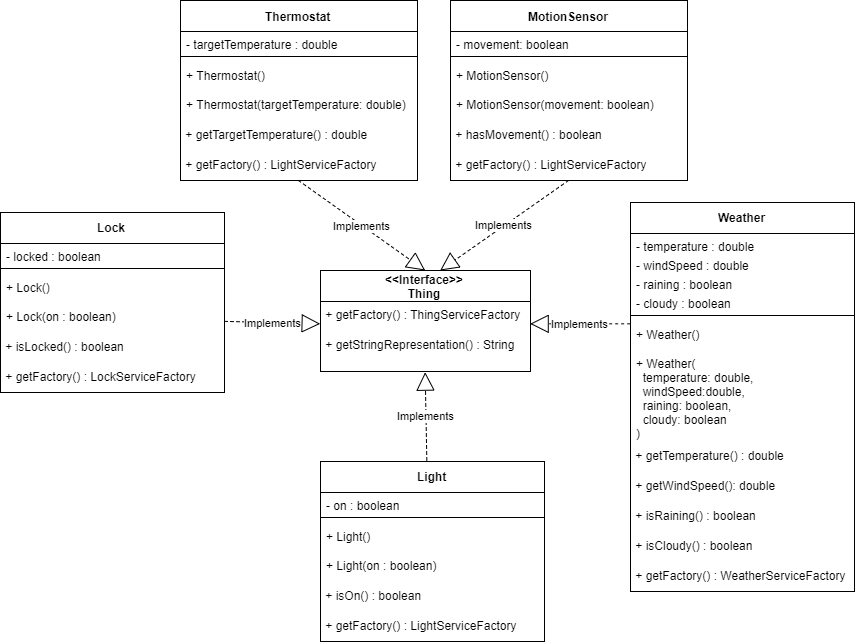
\includegraphics[scale=0.55]{img/hub-things.png}
  \caption{Diagrama de classes: \textit{Things}}
  \label{fig:things-hub}
\end{figure}

%
%
% SERVIÇOS
%
%

\paragraph*{Serviços}

Posto isto, teremos agora que idealizar a comunicação com os dispositivos. Neste caso faremos o uso de serviços, classes que possuem métodos para interagir com um dispositivo específico. Os serviços podem partilhar funcionalidade, como métodos para comunicação HTTP, e portanto esse tipo de funcionalidades estão encapsuladas em classes abstratas auxiliares. Neste caso, além do serviço base, temos também o serviço HTTP e CoAP, que possuem métodos auxiliares para comunicar com dispositivos que utilizem os protocolos respetivos.

Para cada subtipo de uma \textit{thing} deve existir um serviço. Como já vimos anteriormente, um subtipo representa um modelo especifico do dispositivo, e como cada subtipo exige um tipo de comunicação e interação diferente, é portanto necessário ter um serviço para cada um. No diagrama abaixo vemos os serviços para os subtipos da \textit{thing} do tipo \textit{light}, \textit{coap} e \textit{rest}.

\begin{figure}[H]
  \centering
        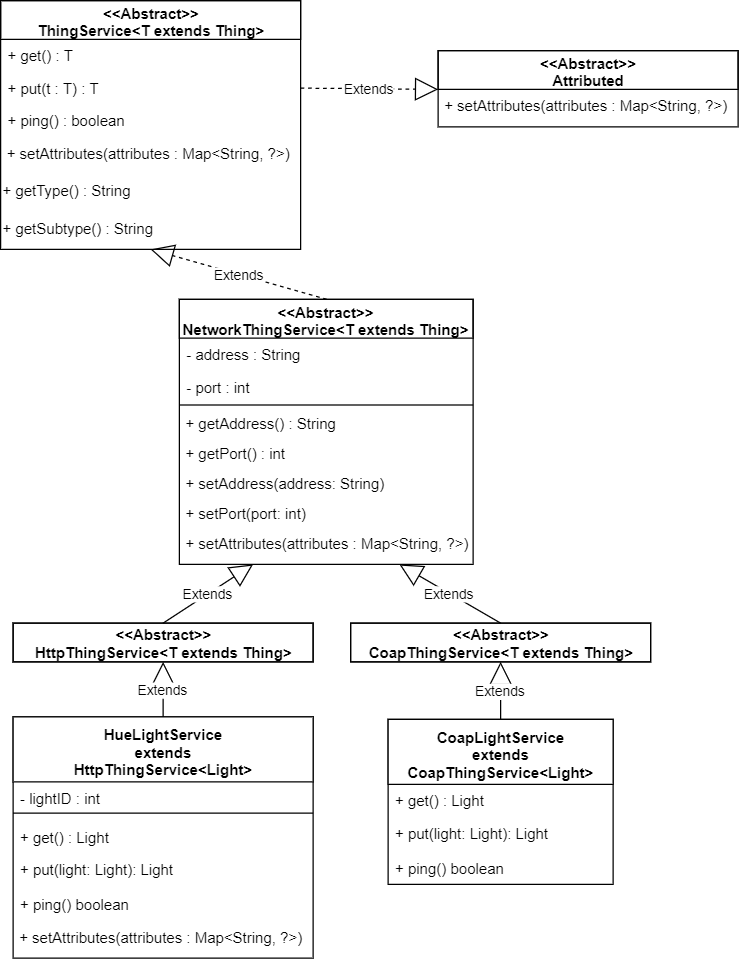
\includegraphics[scale=0.5]{img/hub-services.png}
  \caption{Diagrama de classes: Serviços}
\end{figure}

\newpage

Os restantes serviços serão de seguida enumerados, indicando as classes abstratas em que se baseiam:
\begin{itemize}
    \item \textit{rest light} -> RestLightService -> HttpThingService<Light>
    \item \textit{rest lock} -> RestLockService -> HttpThingService<Lock>
    \item \textit{rest thermostat} -> RestThermostatService -> HttpThingService<Thermostat>
    \item \textit{rest weather} -> RestWeatherService -> HttpThingService<Weather>
    \item \textit{owm weather} -> OWMWeatherService -> ThingService<Weather>
    \item \textit{rest motionsensor} -> RestMotionSensor -> HttpThingService<MotionSensor>
\end{itemize}

Os serviços possuem todos os parâmetros para efetuar comunicação com um dispositivo, nomeadamente o seu endereço, porta de acesso, entre outros. Estes parâmetros são fornecidos ao \textit{hub} nas chamadas à sua API e por ventura são passados aos serviços. O método \textit{setAttributes}, fornecido pela classe abstrata \textit{Attributed}, aceita um \textit{array} associativo, ou por outras palavras, um \textit{map}, que contém todos os atributos necessários para o seu funcionamento. Caso faltem atributos ou estes tenham formatos inválidos, deverá ser lançado um erro, uma exceção, ou um qualquer mecanismo da linguagem para assinalar \textit{inputs} inválidos. Apesar dos \textit{setters} e dos \textit{getters} presentes nos serviços, este método permite definir os atributos tendo apenas uma instância de \textit{ThingService}, sem saber a classe concreta da instância.

As instâncias concretas dos serviços não são de acesso público, apenas o interface base e as extensões abstratas. Decidiu-se proceder desta maneira para reduzir o acoplamento entre os serviços e as outras partes da aplicação, nomeadamente os \textit{controllers} que recebem parâmetros das chamadas à API e que comunicam com os dispositivos, utilizando os serviços para isso. Assim sendo, todos os serviços serão instanciados através de \textit{factories}, que recebem um subtipo e devolvem uma instância dum serviço referente ao subtipo dado. Mais uma vez, é por esta razão que definiu-se o método \textit{setAttributes}, para efetuar o \textit{assign} dos atributos sem ter acesso à classe específica de uma instância de um serviço.

A classe auxiliar \textit{Attributed}, em termos lógicos, basicamente assinala isto que já foi exposto, uma classe que permite mudar o seu estado interno, ou por outras palavras, os seus atributos, através de um \textit{map} entre o nome do atributo e o seu valor. Este comportamento foi extraído do serviço porque é utilizado noutros pontos da aplicação, nomeadamente a descoberta de serviços, que utiliza este mecanismo pelas mesmas razões supracitadas.

Os dispositivos do tipo base \textit{NetworkThingService} requerem todos um endereço e uma porta, que poderão ser passados à instância de um serviço através dos seus \textit{setters}, no entanto, não podemos fazer tal coisa, porque apenas interagimos com instâncias do tipo \textit{ThingService}, devido ao acesso privado das classes concretas. Para resolver isso utilizamos o método \textit{setAttributes}, como já se falou anteriormente. Classes que recorrem a parâmetros adicionais, como o \textit{HueLightService}, que faz uso do novo parâmetro \textit{lightID}, devem voltar a implementar o método \textit{setAttributes} para acomodar o novo parâmetro.

%
%
% FACTORIES
%
%

\paragraph*{\textit{Factories}}

Devido à abordagem à base de ''um serviço para um subtipo'', iremos ter várias classes concretas para cada um dos subtipos de dispositivos, portanto, irá ser utilizado o padrão \textit{abstract factory}, onde teremos várias fábricas de serviços, uma por cada tipo de dispositivo, para simplificar o processo de instanciação de serviços. Por exemplo, a fábrica do tipo ''luz'' é responsável por instanciar todos os serviços suportados por este tipo de dispositivo, aceitando um subtipo como parâmetro. As fábricas de objetos também devem ter um método de utilidade para ver se um dado subtipo é suportado. Além disso, o método \textit{create} deve, obviamente, finalizar com um erro quando o subtipo não é suportado.

\begin{figure}[H]
  \centering
        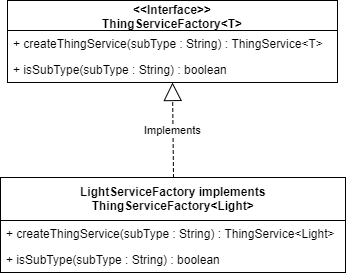
\includegraphics[scale=0.75]{img/hub-factories.png}
  \caption{Diagrama de classes: \textit{Factories}}
\end{figure}

Neste diagrama apenas está representada a \textit{LightServiceFactory}, mas todos os outros tipos de dispositivos tem fábricas com assinaturas semelhantes. O método \textit{create} retorna os serviços definidos acima, mas sem exportar os detalhes da classe concreta. Caso o método \textit{create} seja chamado com o subtipo \textit{hue} numa fábrica do tipo \textit{LightServiceFactory} a fábrica retorna um \textit{HueLightService} abstraído no interface \textit{ThingService<Light>}.

O interface base \textit{ThingServiceFactory} irá ter uma função vital nos \textit{controllers}, permitindo efetuar \textit{dependency injection} nestes, simplificando a operação dos mesmos. Assim, um \textit{controller} genérico consegue operar com qualquer tipo de dispositivo, baseado na \textit{factory} que o compõe.

%
%
% CONTROLLERS
%
%

\paragraph*{Controllers}

Seguindo a arquitetura MVC, já temos os componentes que representam o \textit{model}, neste caso as \textit{things} e os serviços, restando os \textit{controllers} e as \textit{views}. Os \textit{controllers} têm como função aceitar parâmetros provenientes da chamada à API, gerando alterações nos \textit{models}, ou mais concretamente, nos dispositivos. Além de gerar alterações, os \textit{controllers} também podem gerar as tais \textit{views}, representações dos estados dos dispositivos.

Tal como foi explicado no \textit{design} das \textit{factories}, os \textit{controllers} irão funcionar à base de \textit{dependency injection}, sendo compostos por uma \textit{ThingServiceFactory}, que irá ditar o tipo de dispositivos com que o \textit{controller} lida. Assim, tendo apenas uma definição base de um \textit{controller}, conseguimos trabalhar com todo o tipo de dispositivos, em vez de criar um \textit{controller} para cada tipo individual. Todo o objetivo de lidar com os genéricos, que consistem nestas classes parametrizadas com um tipo genérico \textit{T}, é atingir esta abstração, onde um \textit{controller} consegue lidar com vários tipos e subtipos de dispositivos, abstraindo todo este processo de seleção de serviços e passagem de parâmetros.

\begin{figure}[H]
  \centering
        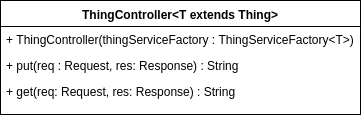
\includegraphics[scale=0.75]{img/hub-controllers.png}
  \caption{Diagrama de classes: \textit{Controllers}}
\end{figure}

O \textit{ThingController} é instanciado com uma \textit{ThingServiceFactory}, e possui dois métodos, \textit{get} e \textit{put}, que correspondem aos verbos HTTP GET e PUT, seguindo assim uma metodologia \textit{restful}, onde temos os recursos (\textit{things}) e utilizamos verbos HTTP para interagir com os recursos. O método \textit{put} tem como objetivo alterar o estado de um dispositivo dado um \textit{request} e uma \textit{response}, objetos que representam um pedido e uma resposta HTTP, normalmente de uma \textit{framework} de desenvolvimento de servidores web. O método \textit{get} serve apenas para retornar o estado atual de um dispositivo. Ambos estes métodos retornam uma \textit{string}, que representa a resposta da API em JSON a um qualquer pedido.

Internamente, o \textit{controller} recebe um pedido, retira o parâmetro subtipo dos parâmetros deste, cria um serviço através da \textit{factory}, utiliza o método \textit{setAttributes} atribuindo os restantes parâmetros, e depois chama o método correspondente no serviço, ou \textit{get} ou \textit{put}.

\newpage

%
%
% Descoberta de dispositivos
%
%

\paragraph*{Descoberta de Dispositivos}

Posto isto, temos os serviços que permitem estabelecer comunicação bidirecional com os dispositivos, faltando agora resolver o problema da descoberta de dispositivos na rede local. Uma parte muito importante de todo o paradigma da IoT e do espaço casa, uma vez que aumenta muito a facilidade de uso destes sistemas para o utilizador comum.

Inicialmente foram concebidas as classes para a descoberta de dispositivos, tendo como base o padrão \textit{strategy}, que define estratégias diferentes para resolver um dado problema. Isto traduz-se para uma classe abstrata base com um método \textit{perform}, que essencialmente leva a cabo a descoberta de dispositivos, utilizando uma fábrica de serviços e um subtipo como argumentos (passados através de um construtor).

As estratégias essencialmente dependem do subtipo de dispositivo utilizado. Dispositivos diferentes têm estratégias diferentes de descoberta, alguns podem utilizar UPNP, outros não, sendo necessário encontrar outras alternativas. Utilizando esta abordagem, é alcançável a elaboração de estratégias para cada um dos subtipos, mantendo esse processo transparente noutras camadas da aplicação, nomeadamente os \textit{controllers}.

\begin{figure}[H]
  \centering
        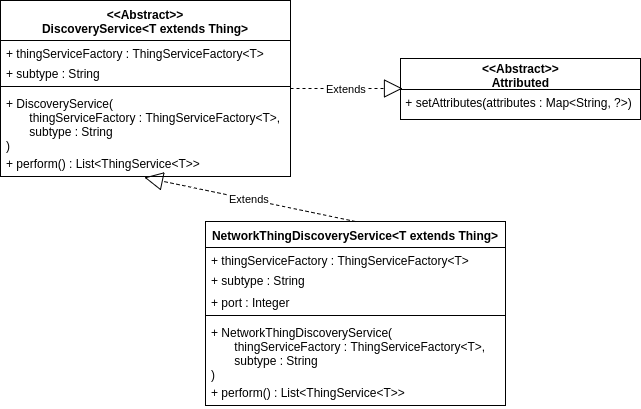
\includegraphics[scale=0.6]{img/hub-discovery.png}
  \caption{Diagrama de classes: \textit{Serviços de descoberta de dispositivos}}
\end{figure}

Neste caso apenas possuímos um único serviço de descoberta, \textit{NetworkThingDiscoveryService}, que descobre todo o tipo de dispositivos baseados no \textit{NetworkThingService}, ou seja, dispositivos que essencialmente atuam utilizando o protocolo IP, ou protocolos que se baseiam neste anterior, como HTTP ou CoAP, estando presentes na rede local do \textit{hub}. O \textit{NetworkThingDiscoveryService}, além do subtipo, que é necessário para todo o tipo de descobertas, também necessita de uma porta. Caso uma porta não seja passada como parâmetro será utilizada a porta ''default'' do protocolo utilizado (HTTP utiliza a porta 80 por exemplo).

Todos os subtipos são cobertos por esta estratégia de descoberta, exceto um, o subtipo \textit{owm}, que como se baseia num serviço remoto, não necessita de mecanismos de descoberta.

Concebida a arquitetura dos serviços, é preciso unir tudo e criar um \textit{controller} para expor esta funcionalidade, mas antes disso, ainda falta resolver de alguns detalhes. Primeiro, está novamente presente o problema encontrado nos \textit{thing services}, onde temos vários objetos distintos, tornando a sua instanciação um processo complexo. Para resolver isto, basta adicionar um outro método às \textit{factories}, que devolve uma implementação de um \textit{DiscoveryService} compatível com o \textit{subtipo}.

\begin{figure}[H]
  \centering
        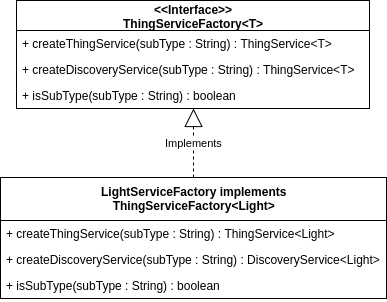
\includegraphics[scale=0.6]{img/hub-factories-discovery.png}
  \caption{Diagrama de classes: \textit{Factories atualizadas para suportar serviços de descoberta}}
\end{figure}

Assim, temos um mecanismo para obter a estratégia de descoberta de um determinado subtipo, simplificando todo esse processo da escolha da estratégia num novo método nas \textit{factories}. Os \textit{controllers} então só têm que trabalhar com instâncias de \textit{DiscoveryService}, utilizando o método \textit{setAttributes} da classe abstrata \textit{Attributed} para passar os parâmetros recebidos pelo \textit{controller}.

Por fim, efetua-se a conceção dos \textit{controllers} que expõem os serviços de descoberta. Estes \textit{controllers}, têm um funcionamento muito semelhante aos \textit{controllers} dos serviços das \textit{things}. Este tipo de \textit{controllers} só possui suporte para métodos do tipo GET, retornando uma lista de dispositivos disponíveis na rede local, e os parâmetros necessários para o seu funcionamento.

%depois mostramos como integramos isto num todo, mostrando o controller

O \textit{controller} extrai o subtipo fornecido nos parâmetros, utilizando a \textit{factory} para criar o \textit{discovery service} correspondente ao subtipo. Depois disto, são passados o restos dos parâmetros, como a porta de acesso no caso dos \textit{NetworkThingDiscoveryService}, utilizando o método \textit{setAttributes}. Por fim, após esta passagem de parâmetros é então executado o método \textit{perform} do serviço de descoberta, retornando a lista de dispositivos encontrados na rede do \textit{hub}.

%
%
% VISAO GERAL
%
%

\paragraph*{\textit{API HTTP} - Visão Geral}

Concluindo o desenho arquitetural, agora prossegue-se à definição da API HTTP que irá ser consumida pelo \textit{core} do \textit{middleware}.

Uma API HTTP é normalmente constituída por recursos, identificados por um URL, e pelas ações disponíveis em cada um. Uma ação é identificada pelo verbo HTTP, como já foi demonstrado no \textit{design} dos \textit{controllers}. Exemplos de verbos HTTP podem ser o GET, que tem como função a simples obtenção de um recurso, e o PUT, que tem como função a alteração de um recurso existente.

Posto isto, temos primeiros os URLs de acesso aos dispositivos, cada um com suporte para operações GET e PUT, onde o GET retorna o estado do dispositivo e o PUT permite alterar o estado do dispositivo.

\begin{verbatim}
            /devices/lights
            /devices/locks
            /devices/thermostats
            /devices/weather
            /devices/motionsensors
\end{verbatim}

Os parâmetros de acesso, como o endereço IP do dispositivo, devem ser passados à API através de uma \textit{query string}, adicionada ao URL. Estes parâmetros são recolhidos pelo \textit{controller} e posteriormente passados para os serviços respetivos, quer os serviços das \textit{things} ou de descoberta.

\begin{verbatim}
            /devices/light?subtype=rest&address=foo.light.local&port=80
\end{verbatim}

Este exemplo permite estabelecer contacto com um dispositivo do tipo \textit{light} e do subtipo \textit{rest}, utilizando o endereço \textit{foo.light.local} e a porta 80 como parâmetros de rede. Internamente, este pedido e os seus parâmetros são passados ao \textit{ThingController} e depois este trata de completar a operação em causa.

Com ambos os verbos HTTP, a resposta a uma chamada da API do \textit{hub} é um objeto do tipo \textit{thing} serializado para JSON. O corpo dos pedidos do tipo PUT também deve seguir a mesma estrutura e formato. De seguida podemos observar um objeto do tipo \textit{light} no formato JSON.

\begin{verbatim}
            {
                "on" : false
            }
\end{verbatim}

Todas as variáveis de instância de qualquer \textit{thing} são convertidas na serialização, de modo a que as restantes representações em JSON dos outros tipos podem ser inferidas através da figura \ref{fig:things-hub}.

As rotas para interagir com os serviços de descoberta têm o seguinte formato:

\begin{verbatim}
            /devices/lights/discover
            /devices/locks/discover
            /devices/thermostats/discover
            /devices/weather/discover
            /devices/motionsensors/discover
\end{verbatim}

Para encontrar um dispositivo basta efetuar um pedido GET para uma destas rotas, fornecendo como parâmetros um subtipo mais outro subconjunto de parâmetros dependendo do subtipo em questão.

\begin{verbatim}
            /devices/light/discover?subtype=rest&port=80
\end{verbatim}

Este pedido procura por dispositivos do tipo \textit{rest} que estejam a operar na porta 80. Um exemplo de resposta tem o seguinte formato:

\begin{verbatim}
            [
                {
                    "address":"foo.light.local",
                    "port":80,
                    "subtype":"rest",
                    "type":"Things::Light"
                }
            ]
\end{verbatim}

Basicamente trata-se de uma lista JSON com os dispositivos encontrados. Internamente são os serviços que são serializados para JSON, serializando os atributos relevantes ao funcionamento do serviço, neste caso \textit{address}, \textit{port}, \textit{subtype} e \textit{type}.